\chapter{Badanie obiektu}
\section{Symulacja różnych odpowiedzi skokowych obiektu}

Poniżej zamieszczono kod programu przeprowadzającego symulację obiektu dla ustalonegych $u$  z przedziału $ \langle  U^{\textrm{min}}, U^{\textrm{max}}\rangle $ uzyskując różne odpowiedzi skokowe. 

\begin{lstlisting}[style=Matlab-editor, basicstyle=\tiny]
t_sim2 = 300;

%konstruowanie sygnalow sterujacych
step_tim = 0;

u_base = ones(1,step_tim)*u_pp;
u_step_temp = ones(1,t_sim2 - step_tim)*1.3;
u_step2_temp = ones(1,t_sim2 - step_tim);
u_step3_temp = ones(1,t_sim2 - step_tim)*1.6;

u_step = [u_base, u_step_temp];
u_step2 = [u_base, u_step2_temp];
u_step3 = [u_base, u_step3_temp];

y = ones(t_sim2, 1)*y_pp;
y2 = ones(t_sim2, 1)*y_pp;
y3 = ones(t_sim2, 1)*y_pp;

for k = 3:t_sim2
    if k-11 <= 0
        y(k) = symulacja_obiektu6Y(u_pp,u_pp,y(k-1),y(k-2));
        y2(k) = symulacja_obiektu6Y(u_pp,u_pp,y2(k-1),y2(k-2));
        y3(k) = symulacja_obiektu6Y(u_pp,u_pp,y3(k-1),y3(k-2));
    else
        y(k) = symulacja_obiektu6Y(u_step(k-10),u_step(k-11),y(k-1),y(k-2));
        y2(k) = symulacja_obiektu6Y(u_step2(k-10),u_step2(k-11),y2(k-1),y2(k-2));
        y3(k) = symulacja_obiektu6Y(u_step3(k-10),u_step3(k-11),y3(k-1),y3(k-2));      
    end
end
\end{lstlisting}

W wyniku przeprowadzenia symulacji, otrzymano następujące przebiegi:
\begin{figure}[h] 
\centering 
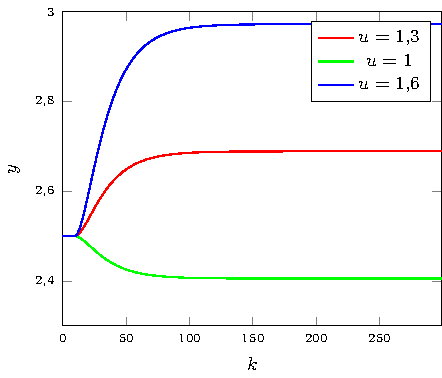
\includegraphics[scale=1.4]{wykresy/zad1_2/2_1.pdf} 
\caption{Odpowiedzi układu dla ustalonegych $u$  z przedziału $ \langle  U^{\textrm{min}}, U^{\textrm{max}}\rangle $ } 
\end{figure}

\par Na pierwszy rzut oka, obiekt wydaje się mieć liniową strukturę. Aby jednak to potwierdzić, należy wyznaczyć charakterystykę statyczną.


\section{Charakterystyka statyczna}
Aby wyznaczyć charakterystykę statyczną, stworzono symulację dla równiomiernie rozłożonych wartości sterowania z zakresu $ \langle  U^{\textrm{min}}, U^{\textrm{max}}\rangle $. Dla każdej z wartości sterowania wykonywano skok, a następnie czekano, aż wartość sygnału wyjściowego się ustabilizuje. Kod symulacji zamieszczony został poniżej:

\begin{lstlisting}[style=Matlab-editor]
t_sim = 400;
y_wyj = [];

for u = 0.6:0.01:1.6
    y = [0;0];
    for k=2:t_sim
        y_temp = symulacja_obiektu6Y(u,u,y(k),y(k-1));
        y = [y;y_temp];
    end
    y_wyj = [y_wyj; y(end)];
end
\end{lstlisting}

Poniżej zaprezentowany został wynik symulacji:
\begin{figure}[h] 
\centering 
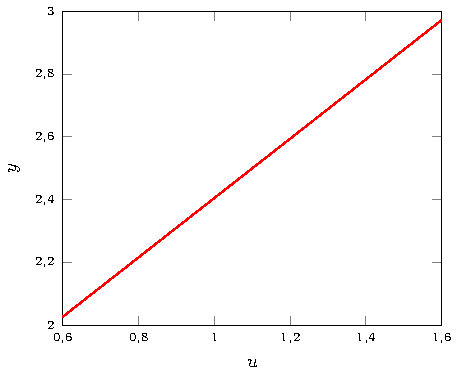
\includegraphics[scale=1.4]{wykresy/zad1_2/char_stat.pdf} 
\caption{Przybliżona charakterystyka statyczna układu} 
\end{figure}
Wyraźnie widać, że charakterystyka statyczna obiektu jest liniowa. Można zatem obliczyć wzmocnienie statyczne obiektu mając na uwadzę zależność:

\begin{equation}
K_{\textrm{stat}} = \frac{Y^{\textrm{max}} - Y^{\textrm{min}}}{U^{\textrm{max}} - U^{\textrm{min}}}
\end{equation}
Na podstawie powyższych rozważań obliczono $K_{\textrm{stat}} = \num{0.936}$



